% Copyright (c) 2008-2009 solvethis
% Copyright (c) 2010-2016,2018-2019,2021 Casper Ti. Vector
% Copyright (c) 2021 Kurapica
% Copyright (c) 2021 iofu728
% Overleaf version.

%*********************************************************************
% iofu728-pkuthss: 北京大学研究生学位论文模板
% 2021/06/09 v1.0.0
%
% 重要提示:
%   1. 当前overleaf版符合2021研究生学位论文要求,可通过图书馆审核
%   2. 当前版本基于pkuthss v1.9.0
%   3. 请使用UTF-8编码,XeLaTeX方式编译
%   4. 请仔细阅读用户文档
%   5. 修改、使用、发布本文档类请务必遵循LaTeX Project Public License和知识共享4.0
%   6. 如有疑问github/iofu728/pkuthss上提问或联系作者@iofu728
%*********************************************************************

\documentclass[fontset=fandol,ugly]{pkuthss}
  % 学位论文模式  ugly    (默认打开,请保留)
  % 盲审模式      blind   (默认关闭)
  % 字体库        fontset
  %   auto | windows | windows@overleaf | mac | fandol | ubuntu | none
  % windows*, mac为商业字体,如需使用请遵循相应版权协议(默认下overleaf中不可用)
  % fandol与windows效果相近,但字符库偏少,推荐使用(默认);
  % ubuntu字体效果偏差较大; 设为none时需自行配置字体集;

\usepackage[backend=biber,style=gb7714-2015]{biblatex}
  % 参考文献遵循GB/T 7714-2015标准,使用biblatex-gb7714-2015 宏包。
  % 此处使用顺序编码制,如使用著者-出版年制则更改为b7714-2015ay。

% 示例文档用包和设定,该段均可移除.
\usepackage{enumitem,fancyvrb}
\usepackage{booktabs,multirow,longtable,makecell} % 表格相关
\RecustomVerbatimEnvironment{Verbatim}{Verbatim}{frame = single, tabsize = 4, fontsize=\footnotesize}
\renewcommand{\v}[1]{\boldsymbol{#1}}
\newcommand\pkg[1]{\textsf{#1}}

% 参考文献边距字体
\setlength{\bibitemsep}{3bp}
\renewcommand*{\bibfont}{\zihao{5}\linespread{1.27}\selectfont}

\pkuthssinfo{
	cthesisname = {密码编码学与网络信息安全期末作业},
 	thesiscover = {密码编码学与网络信息安全期末作业},
	ethesisname = {Homework},
	ctitle = {密码编码学与网络信息安全报告准备},
	etitle = {Homework},
	cauthor = {干皓丞}, eauthor = {Kan, Hao-Cheng},
	studentid = {2101212850},
	% 具体时间以教务为准,初稿3月,送审4月,答辩5月,最终6月。
	%date = {\zhdigits{2021}\ \ 年\ \ \zhnumber{6}\ \ 月},
	date = {\zhdigits{2022}\ \ 年\ \ \zhnumber{6}\ \ 月},
	school = {信息工程学院},
	cmajor = {计算机应用技术}, emajor = {通信及信息安全技术},
	direction = {通信及信息安全技术},
	%mentorlines = {2}, % 导师个数
	mentorlines = {1}, % 导师个数
	% 副教授 A.P. 讲师 Lec.
	cmentor = {朱跃生\ \ 教授}, ementor = {Prof.\ XXX },
	%cmentor = {XXX\ \ 教授\\YYY\ \ 教授}, ementor = {Prof.\ XXX and Prof.\ YYY},
	ckeywords = {論文精讀,文獻管理,LaTeX},
	ekeywords = {A,B,C,D},
	% 盲审模式参数, 需在documentclass增加blind
	blindid = {XXXXXXXXX}, discipline = {XXXX}
}
\addbibresource{ref.bib}

\begin{document}
	\frontmatter
	\pagestyle{empty}
	\maketitle
	\cleardoublepage
	% 需替换门户版权声明pdf
	%% Copyright (c) 2008-2009 solvethis
% Copyright (c) 2010-2017,2021 Casper Ti. Vector
% Copyright (c) 2021 iofu728
% All rights reserved.
%
% Redistribution and use in source and binary forms, with or without
% modification, are permitted provided that the following conditions are
% met:
%
% * Redistributions of source code must retain the above copyright notice,
%   this list of conditions and the following disclaimer.
% * Redistributions in binary form must reproduce the above copyright
%   notice, this list of conditions and the following disclaimer in the
%   documentation and/or other materials provided with the distribution.
% * Neither the name of Peking University nor the names of its contributors
%   may be used to endorse or promote products derived from this software
%   without specific prior written permission.
%
% THIS SOFTWARE IS PROVIDED BY THE COPYRIGHT HOLDERS AND CONTRIBUTORS "AS
% IS" AND ANY EXPRESS OR IMPLIED WARRANTIES, INCLUDING, BUT NOT LIMITED TO,
% THE IMPLIED WARRANTIES OF MERCHANTABILITY AND FITNESS FOR A PARTICULAR
% PURPOSE ARE DISCLAIMED. IN NO EVENT SHALL THE COPYRIGHT HOLDER OR
% CONTRIBUTORS BE LIABLE FOR ANY DIRECT, INDIRECT, INCIDENTAL, SPECIAL,
% EXEMPLARY, OR CONSEQUENTIAL DAMAGES (INCLUDING, BUT NOT LIMITED TO,
% PROCUREMENT OF SUBSTITUTE GOODS OR SERVICES; LOSS OF USE, DATA, OR
% PROFITS; OR BUSINESS INTERRUPTION) HOWEVER CAUSED AND ON ANY THEORY OF
% LIABILITY, WHETHER IN CONTRACT, STRICT LIABILITY, OR TORT (INCLUDING
% NEGLIGENCE OR OTHERWISE) ARISING IN ANY WAY OUT OF THE USE OF THIS
% SOFTWARE, EVEN IF ADVISED OF THE POSSIBILITY OF SUCH DAMAGE.

% 此处不用 \specialchap,因为学校要求目录不包括其自己及其之前的内容。
\chapter*{版权声明}
% 综合学校的书面要求及 Word 模版来看,版权声明页不用加页眉、页脚。
\thispagestyle{empty}

任何收存和保管本论文各种版本的单位和个人,
未经本论文作者同意,不得将本论文转借他人,
亦不得随意复制、抄录、拍照或以任何方式传播。
否则一旦引起有碍作者著作权之问题,将可能承担法律责任。

% 替换门户下载pdf
\begin{textblock}{1}(-0.8,-0.08)
    \colorbox{white}{
        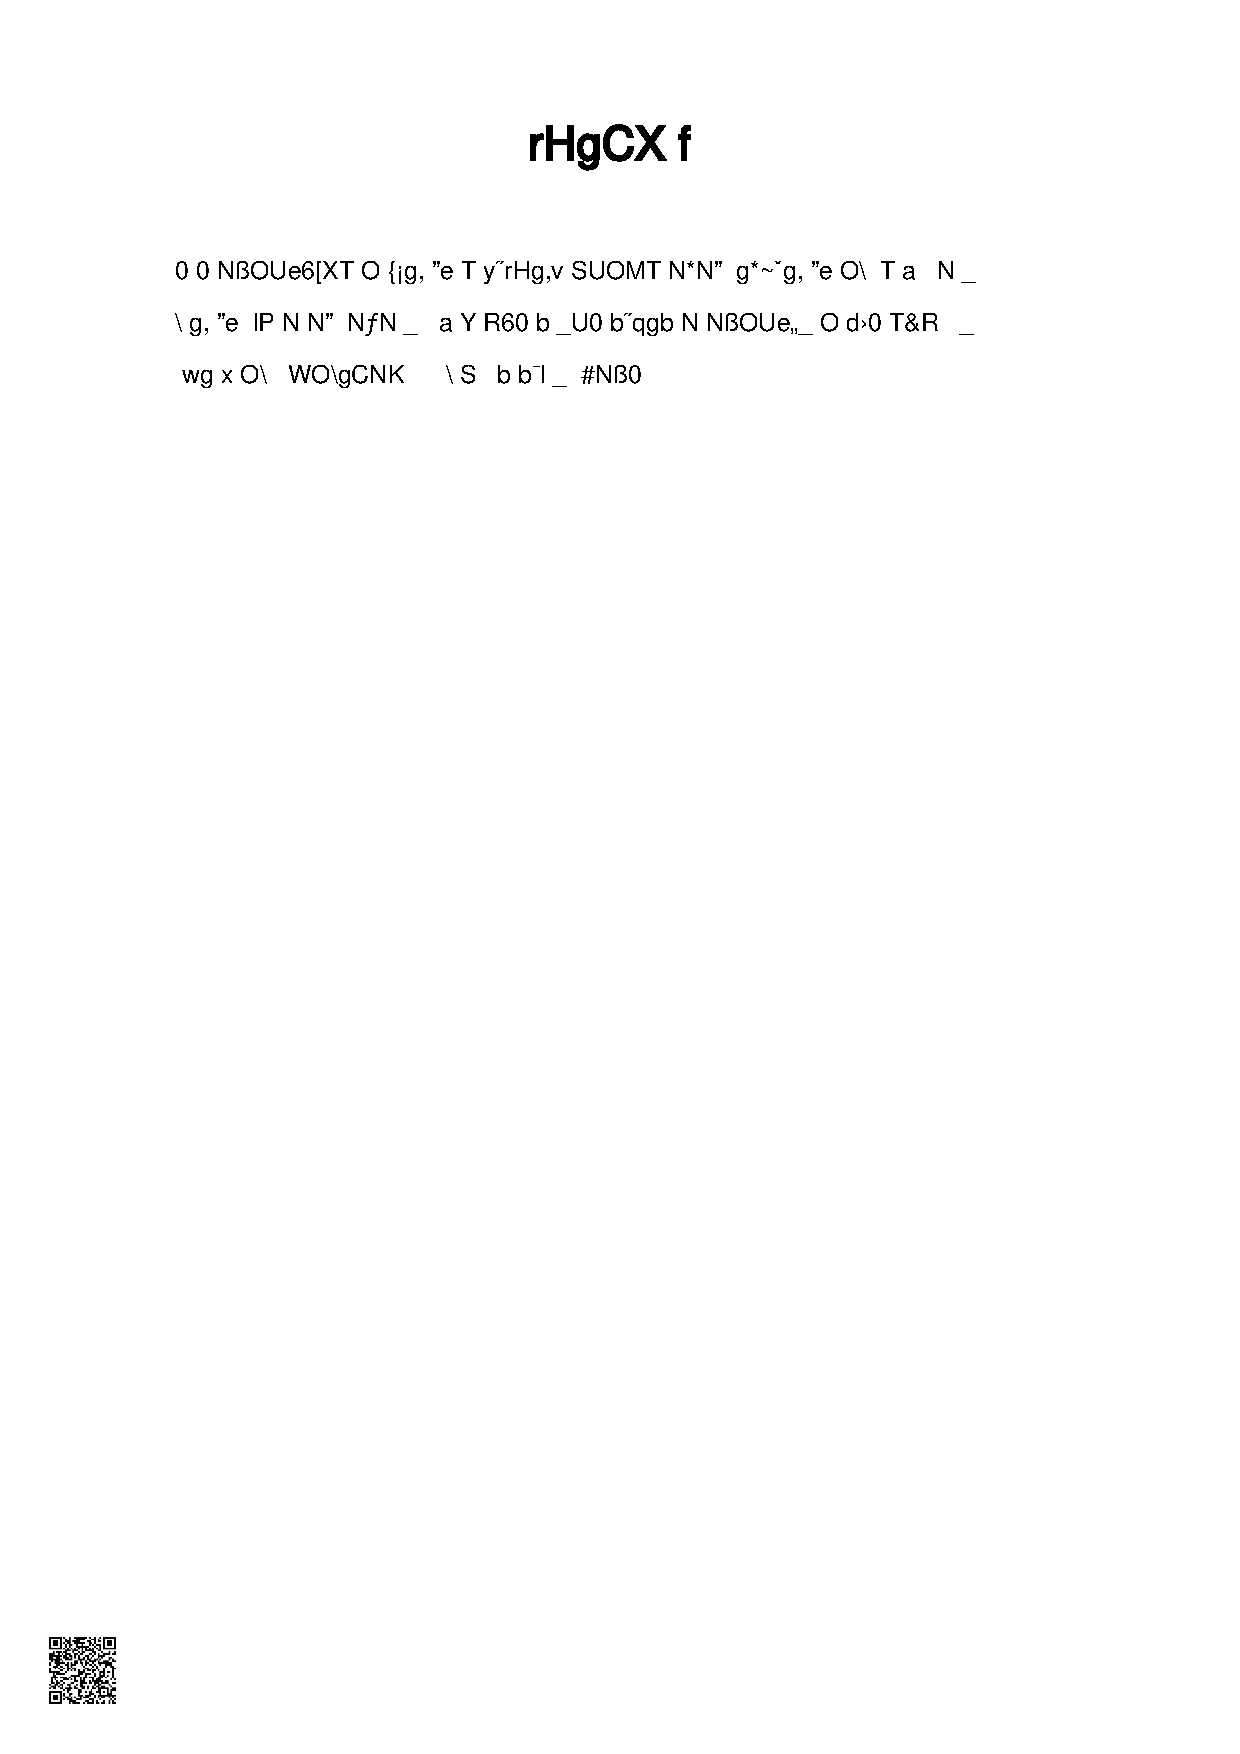
\includegraphics[height = 1.2448\textheight]{img/bqsm_180xxxxxxx.pdf}
    }
\end{textblock}

% vim:ts=4:sw=4

	\cleardoublepage
	\pagestyle{plain}
	\setcounter{page}{0}
	\pagenumbering{Roman}
	\begin{cabstract}

XXXXX


\end{cabstract}

%\begin{eabstract}
%    英文摘要部分...
%\end{eabstract}

% vim:ts=4:sw=4

	\tableofcontents
	% 如有需要使用主要符号对照表
	\begin{denotation}

\item[$x,y,m,n,t$] 标量,通常为变量
\item[$K,L,D,M,N,T$] 标量,通常为超参数
\item[$x\in \mathbb{R}^{D}$] D维列向量
\item[$(x_1,\cdots,x_D)$] D维行向量
\item[$(x_1,\cdots,x_D)^T$ or $(x_1;\cdots;x_D)^T$]  D维行向量
\item[$x\in \mathbb{R}^{KD}$]  ($KD$)维的向量
\item[$\mathbb{M}_i$ or $\mathbb{M}_i(\v x)$]  第$i$列为$\v 1$(或者$\v x$),其余为$\v 0$的矩阵
\item[$diag(\v x)$]  对角矩阵,其对角元素为$\v x$
\item[$\v I_N$ or $I$]  ($N\times N$)的单位阵
\item[$\v A \in \mathbb{R}^{D_1\times D_2\times \cdots \times D_K}$]  大小为$D_1\times D_2\times \cdots \times D_K$的张量
\item[$\{x^{(n)}\}^{N}_{n=1}$]  集合
\item[$\{(x^{(n)},y^{(n)})\}^{N}_{n=1}$]  数据集
\item[$\mathcal{N}(\v x;\mu,\sum)$]  变量$x$服从均值为$\mu$,方差为$\sum$的高斯分布

\end{denotation}

\footnotetext[1]{本符号对照表内容选自\citeauthor{qiu2020nndl}老师的《神经网络与深度学习》\cite{qiu2020nndl}一书。}


	\mainmatter
	\chapter{论文精读}
\label{chap:1}

从下面两处期刊来源,进行翻译、阅读并写出心得,而研究论文来源如下所示 :
% \cite{garcia2020admd}
\begin{Verbatim}
1. IEEE Transactions on Pattern Analysis and Machine Intelligence
(TPAMI) (SCI IF 16.389), 2021.
2. IEEE Journal on Selected Areas in Communications (SCI IF 9.114), 2021.
\end{Verbatim}

而论文心得必须根据 IMRAD 的方式进行撰写,其流程分别为四部分,分别为前言(Introduction)、方法(Methods)、结果(Results)和讨论(Discussion),最后则是根据原论文架构的范例。

\section{论文精读资讯}

下列论文资讯有二 \cite{garcia2020admd} ,其一为 arXiv 的 1810.08437 所示 的资讯,其二为 IEEE Transactions on Pattern Analysis and Machine Intelligence 的公开资讯。

\begin{Verbatim}
1. arXiv
Learning with Privileged Information via Adversarial Discriminative Modality Distillation
Nuno C. Garcia, Pietro Morerio, and Vittorio Murino, Senior Member, IEEE
Comments: Accepted to IEEE Transactions on Pattern Analysis and Machine Intelligence
Subjects: Computer Vision and Pattern Recognition (cs.CV)
Link: https://arxiv.org/abs/1810.08437
2. IEEE Transactions
Published in: IEEE Transactions on Pattern Analysis and Machine Intelligence 
( Volume: 42, Issue: 10, Oct. 1 2020)
Page(s): 2581 - 2593
Date of Publication: 16 July 2019 
ISSN Information:
 - Print ISSN: 0162-8828
 - CD: 2160-9292
 - Electronic ISSN: 1939-3539
PubMed ID: 31331879
INSPEC Accession Number: 19931889
DOI: 10.1109/TPAMI.2019.2929038
Publisher: IEEE
Link: https://ieeexplore.ieee.org/document/8764498
\end{Verbatim}


\section{论文心得}

其论文中文字面意义上为,通过对抗性判别模态蒸馏(Adversarial Discriminative Modality Distillation) 学习特权资讯 (Privileged Information),其该篇有趣的地方在于,此研究者想要判别影像深度的远近,该心得则根据 IMRAD 来分析。

\subsection{前言}
该篇研究者想要判断视觉任务的影像远近,研究者提出了一种针对 RGB-D 视觉任务的新方法,该方法是在对抗性学习和特权资讯框架内开发的。研究者考虑从深度和 RGB 影像中学习表示的实际案例,而在测试时仅依赖于 RGB 资料。研究者报告了 NYUD 资料集上对象分类的最新结果,以及可用于此任务的最大多模式资料集 NTU RGB+D 
以及 Northwestern-UCLA 上的影像动作识别结果。他们提出了一种训练幻觉网络的新方法,该方法通过对抗性学习来学习提取深度资讯,从而产生一种干净的方法,而不会出现一些平衡或超参数损失。深度感知是对 3D 世界进行推理的能力,对许多捕食者的生存至关重要,也是人类理解周围环境并与之互动的重要技能。
\subsection{方法}
研究者提出了一种在多模式流网络架构中学习幻觉网络的新方法,它包含一种对抗性学习策略,该策略在训练时利用多种资料模态,而在测试时仅使用一种。事实证明,它优于基于距离的方法,并且通过对距离度量、资料模态和幻觉特征向量的大小,等组件不可知来增强其灵活性。从技术上来说,该研究提出了一个时间感知的鉴别器网络,并联合解决了两个问题,其一为经典的二元分类任务(真实/生成),其二为一个辅助任务,它固有地赋予了学习特征以鉴别能力。我们在特权资讯场景中报告了用于对象分类任务的 NYUD 资料集,以及用于执行以下任务的大规模 NTU RGB+D 和 Northwestern-UCLA 资料集的结果等动作识别。
\subsection{结果}
在此工作中,研究者引入了一种新技术来利用额外资讯,在训练时以深度图像的形式,在测试时改进仅 RGB 模型。该研究通过对抗性训练幻觉网络来完成的,该网络从教师深度流中学习如何从 RGB 帧编码单眼深度特征。同时在三个不同资料集的对象分类和动作识别任务中,所提出的方法在特权资讯场景中优于以前的方法。此外,研究者幻觉框架在深度嘈杂的情况下非常有效。
\subsection{讨论}
RGB 和影像深度实际上是携带补充资讯。而实际上,双流设置总是比单独使用两个流提供令人惊讶的更好的准确性。

其一、作为额外的证据,尽管其单流组件之一,深度或 RGB,取决于任务和资料集的准确性较低,但多模态集合(即双流)的性能优于单模态集合。其二、 RGB 图像中有(单目)深度资讯,从幻觉流经常恢复并且有时超过其基于深度的教师网络的准确性这一事实中可以明显看出这一点。此外,融合幻觉和 RGB 流总是带来好处,如融合 RGB 和深度的部分。而研究者在 RGB 和深度上训练的双流模型的准确度值,并使用 RGB 和噪声深度资料进行测试。其三、标准监督学习在提取资讯方面存在局限性。而事实上,鉴于有证据表明 RGB 图像中存在可利用的深度资讯,最小化交叉熵损失并不足以完全提取出资讯
为此,研究者需要一个学生-教师对抗框架。其四、仅靠对抗训练是不够的。为二元任务(真实/生成)训练的朴素判别器不足以迫使幻觉网络产生判别特征。辅助判别任务对于提取对给定任务也具有判别力的单眼深度线索是必要的(另一方面,仅辅助任务是不够的,正如 RGB 集成的性能所暗示的那样)。其五、幻觉特定于任务的深度特征比估计全深度图像更有效。不仅估计的深度通常缺少分类所需的细节,而且其估计仅由重建目标驱动。相反,特征幻觉解决了特定的分类任务,需要估计低维向量而不是图像。
\section{论文翻译}

在此根据论文 Learning with Privileged Information via Adversarial Discriminative Modality Distillation 的章节结构进行翻译,其论文题目的中文字面意义上为通过对抗性判别模态蒸馏(Adversarial Discriminative Modality Distillation) 学习特权资讯 (Privileged Information)。该根据原研究论文架构来分配章节,该篇研究的论文程式码可于 GitHub 专案
取得 (https://github.com/pmorerio/admd)。

\subsection{摘要}
%Abstract 摘要

异构资料模式可以为多个任务提供补充线索,通常会导致更强大的演算法和更好的性能。然而,虽然可以准确地收集训练资料以包括各种感官模式,但在现实生活(测试)场景中,通常情况下并非所有这些都可用,在这些场景中必须部署模型。这对来自训练阶段的多模态资料中如何提出讯息提出了挑战,以一种可以在测试时利用的形式,考虑到诸如嘈杂或缺失模态等限制。

本文提出了一种针对 RGB-D 视觉任务的新方法,该方法是在对抗性学习和特权资讯框架内开发的。我们考虑从深度和 RGB 影像中学习表示的实际案例,而在测试时仅依赖于 RGB 资料。我们提出了一种训练幻觉网络的新方法,该方法通过对抗性学习来学习提取深度资讯,从而产生一种干净的方法,而不会出现一些平衡或超参数损失。我们报告了 NYUD 资料集上对象分类的最新结果,以及可用于此任务的最大多模式资料集 NTU RGB+D 以及 Northwestern-UCLA 上的影像动作识别结果。

Index Terms: Multimodal deep learning, adversarial learning, privileged information, network distillation, modality hallucination.

\subsection{前言}
% 1 INTRODUCTION 前言

深度感知是对 3D 世界进行推理的能力,对许多捕食者的生存至关重要,也是人类理解周围环境并与之互动的重要技能。当婴儿开始爬行时,它在人类的早期发育,并从各种机制中出现,这些机制共同促成物体的相对和绝对位置感,称为深度线索。除了双目线索(例如立体视觉),人类还使用与通过阴影、透视、纹理梯度和其他信号(例如,物体越远看起来越模糊的假设,或 如果一个物体遮挡了另一个物体,它必须更近,等等)。事实上,尽管人类在单目视觉设置中低估了物距 [3],但即使遮住一只眼睛,我们仍然能够以良好的效率执行大部分与视觉相关的任务。同样,对于与机器人、自动驾驶、场景理解等相关的许多计算机视觉任务,深度感知通常是最重要的部分。


廉价深度传感器的出现和对大数据的需求导致了包含 RGB、深度、红外和骨架序列的大型多模态资料集,进而刺激了多模态深度学习方法,如果模型考虑其他模式,即深度,而不是仅考虑 RGB 的部分,而传统的计算机视觉任务(如动作识别、对象检测或实例分割)已被证明有助于提高性能。然而在实际场景中部署模型时,由于无法收集足够质量的深度资料(例如,由于远距离或反射问题),预计深度资料并不总是可用是合理的。或到处安装深度传感器,传感器或通信故障,或其他不可预测的事件。


考虑到这个限制,我们想回答以下问题(也在图 1 中描绘):在训练时使用所有可用资料的最佳方法是什么,以便学习稳健的表示,知道存在缺失(或噪声)测试时的模式?换句话说,即使在测试时只有一种模态可用,通过利用多模态资料来训练模型是否有任何附加价值?不出所料,最简单和最常用的解决方案是仅使用将要测试的模态来训练模型。然而更有趣的替代方法是利用可用资料的潜力并使用所有模式训练模型,但要意识到在测试时并非所有模式都可以访问的事实。


这种学习范式,即当模型使用额外资讯进行训练时,通常被称为使用特权资讯学习或使用辅助资讯学习。

\begin{figure}[htb]
\centering 
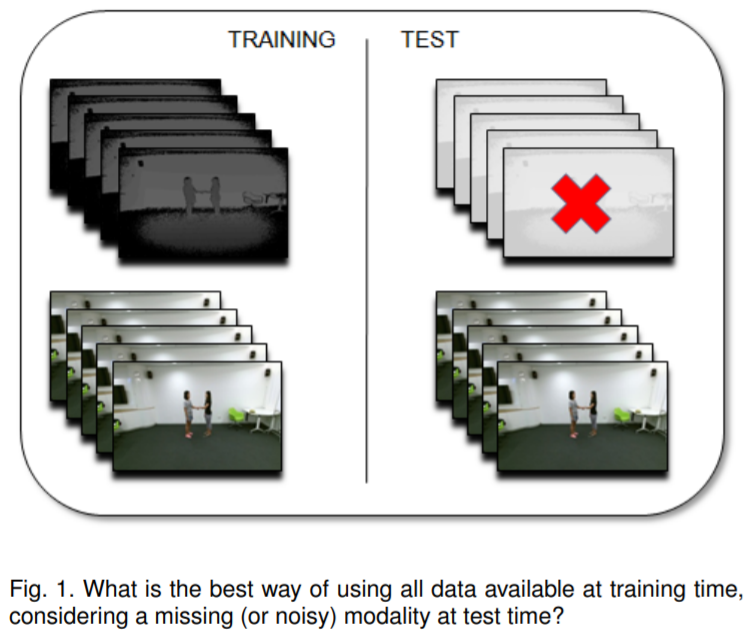
\includegraphics[width=0.80\textwidth]{img/c1m1.png} 
\caption{论文图 1}
\label{Test}
\end{figure}

图 1. 考虑到测试时缺失(或嘈杂)的模态,在训练时使用所有可用资料的最佳方法是什么?

在这项工作中,我们在多模态流框架内提出了一种对抗性判别模态蒸馏 (ADMD) 策略,该策略从不同的资料模态中学习,并且可以在其中的一个子集上进行部署和测试。特别是我们的模型从 RGB 和深度影像序列中学习,并且仅在 RGB 上进行了测试。尽管如此,由于其通用设计,它还可以与其他模式的任何组合一起使用,我们评估其在影像动作识别和对象分类任务上的表现。为此,我们引入了一种新的对抗性学习策略来学习幻觉网络(图 2),其目标是模仿测试时间缺失的模态特征,同时保留其判别力。

幻觉网络仅使用 RGB 作为输入,并尝试为手头的任务恢复有用的深度特征,这种网络可以被认为是上述单眼深度线索的来源,即来自单个 2D RGB 图像的深度线索的来源。我们想强调一个事实,与从 RGB 估计真实深度图相比,我们在特征级别进行操作。从概念上讲,直接从 RGB 估计深度图似乎是在测试时处理缺失深度的更直接的方法。然而,与手头的主要任务(从 RGB 序列识别动作/对象)相比,这可以说是一项更难完成的任务,更合理的方法是将深度估计问题从像素空间减少到低维空间,同时继续在一定程度上受益于深度模态提供的判别优势。

一方面,我们的工作受到以前在特权资讯学习背景下使用幻觉网络的工作的启发,这主要是 J. Hoffman 等人提出的,它提出了一种端到端的单步训练方法来学习幻觉网络,最近在  N. Garcia 中重新审视了这项工作,考虑到使用受广义蒸馏框架,也就是 D. Lopez-Paz 等人所启发的损失的多步学习范式。另一方面,对抗性学习已被证明是对资料分布进行建模的强大工具,基于这些想法,我们提出了一种通过区分性对抗学习策略来学习幻觉网络的新方法。


我们提出的方法有几个优点:它与所使用的模态对无关,这大大简化了它在 RGB 和深度资料之外的扩展; 它能够通过设计来处理影像,利用一种形式的时间监督作为辅助资讯。此外,它不需要平衡其他方法中使用的不同损失。最后,由于鉴别器设计,其中包括一个辅助分类任务,我们的方法能够将鉴别能力从所谓的教师网络(深度网络)转移到学生(幻觉网络),从而达到一个完整恢复老师的准确性。

总而言之,本文的主要贡献如下:

我们提出了一种在多模式流网络架构中学习幻觉网络的新方法:它包含一种对抗性学习策略,该策略在训练时利用多种资料模态,而在测试时仅使用一种。事实证明,它优于基于距离的方法,并且通过对距离度量、资料模态和幻觉特征向量的大小等组件不可知来增强其灵活性。从技术上讲,我们提出了一个时间感知的鉴别器网络,并联合解决了 1)经典的二元分类任务(真实/生成),以及 2)一个辅助任务,它固有地赋予了学习特征以鉴别能力。我们在特权资讯场景中报告了用于对象分类任务的 NYUD 资料集,本文的其余部分安排如下。第 2 节将这项工作与特权资讯、多模态深度学习和对抗性学习方面的文献联系起来。第 3 节介绍了所提出的架构和新颖的学习策略的细节。第 4 节报告了对象识别和影像动作识别资料集的结果,将它们与当前最先进的技术进行比较,最后我们在第 5 节中得出结论和未来的研究方向。

\subsection{相关工作}
% 2 RELATED WORK 相关工作
我们的工作处于四个主题的交叉点:对抗性学习、RGB-D 视觉、网络蒸馏和特权资讯,正如 Lopez et al. 注意到特权资讯和网络蒸馏是相同的更具包容性的理论的实例,并称之为广义蒸馏。

1. 广义蒸馏 (Generalized Distillation)

在广义蒸馏框架内,我们的模型都与特权资讯理论相关,考虑到额外的模态(在这种情况下为深度)仅在训练时使用; 以及蒸馏框架,考虑到我们的幻觉网络通过蒸馏先前学习的“教师”网络的知识而有效地学习,尽管没有使用蒸馏损失。在这种情况下,与我们的方法最接近的作品是 Hoffman et al.。和由 Garcia et al. 撰写,而 Hoffman et al. 的工作,引入了一个模型,用于从 RGB 输入中产生幻觉深度特征,用于对象检测任务,虽然使用幻觉流的想法与由此提出的想法相似,但用于学习它的机制是不同的。

在过往的研究中,作者在深度和幻觉特征图之间使用了欧几里得损失,这是总损失的一部分以及十多个分类和定位损失,这使得它的有效性取决于超参数调整以平衡不同的值,因为模型是通过优化上述复合损失在一步中联合训练的。而 Garcia et al. 基于这个想法,提出了一个新的分阶段训练程序,可以学习更好的教师网
络,以及从蒸馏框架中获得灵感的新损失。

该损失由特征图之间的欧几里得距离、使用真实标签的交叉熵以及使用教师网络(在这种情况下为深度流)的软预测作为目标的交叉熵组成。此外作者鼓励通过设计学习,通过使用乘数交叉流连接,并将方法扩展到影像动作识别,跟过往的研究不同,我们提出了一种对抗性策略来学习幻觉流,这减轻了平衡损失或调整超参数的需要,Neverova et al. 的 ModDrop 是多模态学习和特权资讯学习交叉点的一项有趣工作。

在此作者提出了一种基于模态的 dropout 策略,其中每个输入模态在训练期间以一定的概率被完全丢弃(实际上为零)。结果模型被证明对测试时丢失的模态更有弹性。我们在对象分类的任务中与 ModDrop 进行了比较。罗等人。 Z. Luo 等人解决了一个类似的问题,该模型首先在几种模式(RGB、深度、光流和关节)上进行训练,但仅在一种模式下进行了测试,作者提出了一种基于图的蒸馏方法,可以在训练时从所有模态中提取资讯,允许每种模态向所有其他模态学习。

这种方法在动作识别和动作检测任务中取得了最先进的结果,我们的工作与 Z. Luo 等人有很大不同,因为我们受益于幻觉机制,包括通过利用先前训练的网络训练的辅助幻觉网络,此机制允许模型学习在测试时模拟缺失模态的存在,最近的另一项相关工作是 Y. Zhang 等人,它提出了一个蒸馏框架,其中没有冻结的教师网络,但所有网络都作为一个以协作方式学习的整体工作,此外还探索了使用用于动作识别的特权资讯进行学习的循环神经网络,例如 在 Z. Shi 和 T.-K. Kim 的工作中,作者设计了一种方法,该方法使用骨骼关节作为特权资讯来学习使用深度的更好的动作分类器,即使资料稀少。

2. RGB-D vision RGB-D 视觉

影像动作识别和对象检测拥有悠久而丰富的文献领域,涵盖使用手工特征的分类方法,例如 N. Dalal et al.、H. Wang et al.、I. Laptev et al.、E. S. Ye et al.、S. Tang et al. 、A. Janoch et al. 到现代深度学习方法,例如 S. Gupta et al.、A. Karpathy et al.、D. Tran et al.、X. Wang et al.、A. Wang et al.,仅使用 RGB 或与深度资料一起使用。我们指出了使用 RGB 和深度的影像动作识别和对象识别中一些更相关的工作,包括考虑 NTU RGB+D 和 NYU-Depth V2 资料集的最先进方法,以及我们提出的模型。

(1)  影像动作识别 (Video action recognition)

Simonyan 和 Zisserman 引入的双流模型是影像分析的里程碑,从那时起激发了一系列变体,在不同的资料集上实现了最先进的性能,该架构由 RGB 和光流组成,在此分别训练,然后在预测层融合。我们的模型与此相关,因为测试时间预测来自幻觉流 (the hallucination stream) 和 RGB 流 logits (RGB stream) 的平均值。

在 C. Feichtenhofer et al. 中,作者提出了后者的一种变体,它通过将运动流的信号注入外观流的残差单元来对时空特征进行建模,他们还使用了 1D 时间卷积和 2D 空间卷积,我们在本文中也采用了这种卷积。事实上,2D 空间和 1D 时间卷积的组合已表明比 3D 卷积学习更好的时空特征。当前影像动作识别领域的最新技术是使用 3D 时间卷积和一个新的构建块,专门用于捕获长距离依赖关系,仅使用 RGB 资料,相反的是在过去研究中,作者探索了 RGB 和深度资料的互补特性,将 NTU RGB+D 资料集作为测试平台,他们提出了深度自动编码器架构和结构化稀疏学习机,并在动作识别方面取得了最先进的结果。

Liu et al. 还使用 RGB 和深度设计了一种用于视点不变动作识别的方法,首先该方法从 RGB 资料中提取密集轨迹,然后将其编码为视点不变的深度特征,然后将 RGB 和深度特征用作测试时间预测的字典,据我们所知,这些是利用 RGB+D 进行影像动作识别的最先进方法,在 NTU RGB+D 资料集上报告结果,这是提供 RGB 的最大影像动作识别资料集和深度,需要注意的是,我们提出了一个完全卷积模型,该模型仅在训练时利用 RGB 和深度资料,并在测试时仅使用 RGB 资料作为输入,这项工作的方向是缩小特权资讯与传统方法之间的性能差距。

(2) 物体识别 (Object recognition) 

多年来,基于 RGB 和深度的对象识别一直是推理这两种模式的互补性以及与 RGB 相比是否应该以不同方式处理深度资料的有见地的任务,这方面的一个例子是 S. Gupta et al.,其中作者建议使用地心嵌入对深度图像进行编码,该嵌入对每个像素的地面高度和重力角度以及水平视差进行编码,表明它比使用原始深度效果更好。不同的是在  A. Wang et al. 中,作者专注于精心设计一个卷积神经网络,包括一个多模态层来融合 RGB 和深度,我们的工作与这些方法不同,因为我们专注于学习只能在训练时访问深度的模型,这从根本上改变了特征学习方法。

3. 对抗学习 (Adversarial Learning) 

在 Goodfellow et al. 的开创性论文中,作者提出了一个生成模型,该模型通过让两个网络玩所谓的极小极大游戏来训练,训练生成器网络从噪声向量生成图像,训练鉴别器网络将生成的图像分类为假,并将从资料集中采样的图像分类为真,随着游戏的发展,生成器越来越擅长从资料分布中生成看起来像真实图像的样本。许多论文在不同的方向上扩展了这种方法,例如解开语义概念、网络压缩、特征增强、图像到图像翻译,并探索了不同的损失 和其他提高性能和稳定性的技巧,我们的工作与这一系列工作有关,因为我们模型的幻觉网络试图通过对抗性学习从缺失的模态特征空间中生成特征。然而,不仅这里的上下文不同,因为对抗性学习是在特权资讯的框架中探索的,而且分配给鉴别器的任务也不是对抗性学习中通常使用的任务,如第 3 节所述。

GAN 框架的一个重要变体是条件 GAN(CGAN),它建议将要生成的所需类别的标签连接到噪声向量,这种机制与我们的生成器网络在这项工作中的隐式条件有关,但又有所不同。我们的生成器网络输入是 5 个 RGB 帧的小体积,并且时间卷积被零填充以保持体积沿时间维度的大小。因此,生成器隐含地知道时间顺序,因为为第一帧和最后一帧生成的特征将严重受到零填充的边界效应的影响,零填充会执行多次(在每个残差块),为了解决这个问题,我们还为鉴别器提供了时间排序条件标签。 CGAN 模型已用于不同领域,从图像合成到域适应,也许与我们的工作更相似的是 Roheda et al. 最近的论文,这也解决了在对抗性学习中缺少模态的问题。

它们使用图像、地震和声学传感器解决人员检测的二元任务,而后两者在测试时不存在,CGAN 以可用图像为条件,生成器将矢量噪声映射到来自缺失模态的代表性资讯,并带有辅助 L2 损失。与这项工作相比,我们的 CGAN 模型直接从测试模态到缺失模态的特征空间学习映射,没有辅助损失。此外我们提出了一个两步训练程序,以学习更好的教师网络,并为生成器提供一个稳定的目标。最后,我们专注于影像动作识别和物体识别的要求更高的任务。

\subsection{学习幻觉深度特征}
% 3 LEARNING TO HALLUCINATE DEPTH FEATURES 学习幻觉深度特征

我们的目标是训练一个幻觉网络,该网络以 RGB 为输入,能够产生与深度网络产生的特征相似的特征,这个想法背后的原因是,一方面深度和 RGB 为任务提供了补充资讯,但另一方面,RGB 本身就包含一些深度感知的线索,因此幻觉网络的目标是从 RGB 帧中提取深度资料将提供的补充资讯,需要强调的是,与从 RGB 估计真实深度图相比,我们对恢复有用的深度特征感兴趣,这是在两步训练过程中完成的,如图 2 所示,并在下面描述。

第一步 (图 2,顶部)包括分别训练 RGB 和深度流,使用各自的输入模态,作为两个标准的、独立的、有监督的学习问题。通过融合两个子网络的预测(未微调)获得的最终集成代表了在测试时两种模式都可用时可以使用的完整模型(双流),它的准确性应作为我们提出的模型的上限。在第二步(图 2,底部)中,我们实际上是通过提出的对抗性学习策略来训练幻觉网络。

由于幻觉网络是在对抗性学习的背景下训练生成深度特征的,因此也可以解释为传统 GAN 框架中的生成器网络。然而,严格来说,它显然被认为是一个编码器,它试图从 RGB 输入资料中提取单眼深度特征。步骤 2 的测试时间设置同样是一个双流模型(未微调),由 RGB 和幻觉网络组成,两者都以 RGB 资
料作为输入。

1. 培训程序 (Training procedure) 

受广义蒸馏范式的启发,我们遵循分阶段学习程序,其中首先训练“教师”网络 (步骤 1) 并与“学生”网络分开 (步骤 2),这与  J. Hoffman et al. 形成对比,其中一切都是端到端学习的,但与 N. Garcia et al. 一致,其中分离的学习步骤被证明更有效。

步骤 1. RGB 和深度流分别训练,这是双流架构中的常见做法,在使用预训练的 ImageNet 模型初始化所有实验后,深度和外观流都是通过最小化交叉熵损失来训练的,作为常见做法。

我们分别测试两个流并在双流设置中测试,其中最终预测结果来自两个流的 logits 的平均值,发现微调双流模型并不能始终如一地提高性能。这一步也可以看作是训练教师网络—深度流—用于下一步(见图 2,顶部),步骤 2. 上一步训练的深度流 Ed 现在被冻结,以便为幻觉网络(生成器) H 提供一个稳定的目标,它与判别器 D 进行对抗性游戏 (见图 2,底部)。

步骤 2. 上一步训练的深度流 $E_{d}$ 现在被冻结,以便为幻觉网络(生成器)H 提供一个稳定的目标,它与判别器 D 进行对抗性游戏(见图 2,底部)

鉴别器 D 的主要任务是区分幻觉网络 H 生成的特征 $F_{H}$ 和深度网络 Ed 生成的特征 $F_{d}$,然而正如已经提到的,鉴别器也被分配了一个辅助鉴别任务,如下详述,网络 $E_{d}$ 和 H 的架构是 2D 和 3D 卷积的混合,它们处理一组帧,并为输入卷的每一帧 t 输出一个特征向量,即 $F^{t}_{H}$ 和 $F^{t}_{d}$。

这意味着每一帧都有一个相应的特征向量,即使从同一影像中采样,这些特征向量也可能会有所不同,这取决于其动态及其在输入体积中的位置 t,例如属于“握手”动作的剪辑的第一帧(和特征向量)可能与其中间帧非常不同,但类似于属于“推他人”类的剪辑的第一帧。这增加了生成器的复杂性,它不仅要生成类似于 $F_{d}$ 的特征,还要匹配它们生成的顺序,亦即对于输入体积的每一帧 t,$F_{tH}$ 应该类似于 $F_{td}$,我们通过向 D 提供相对索引 t 的 one-hot 编码向量作为输入来缓解这个问题,我们表示 $y^{t}$,与各自的特征向量连接,这与 CGAN 机制有关,

\begin{figure}[htb]
\centering 
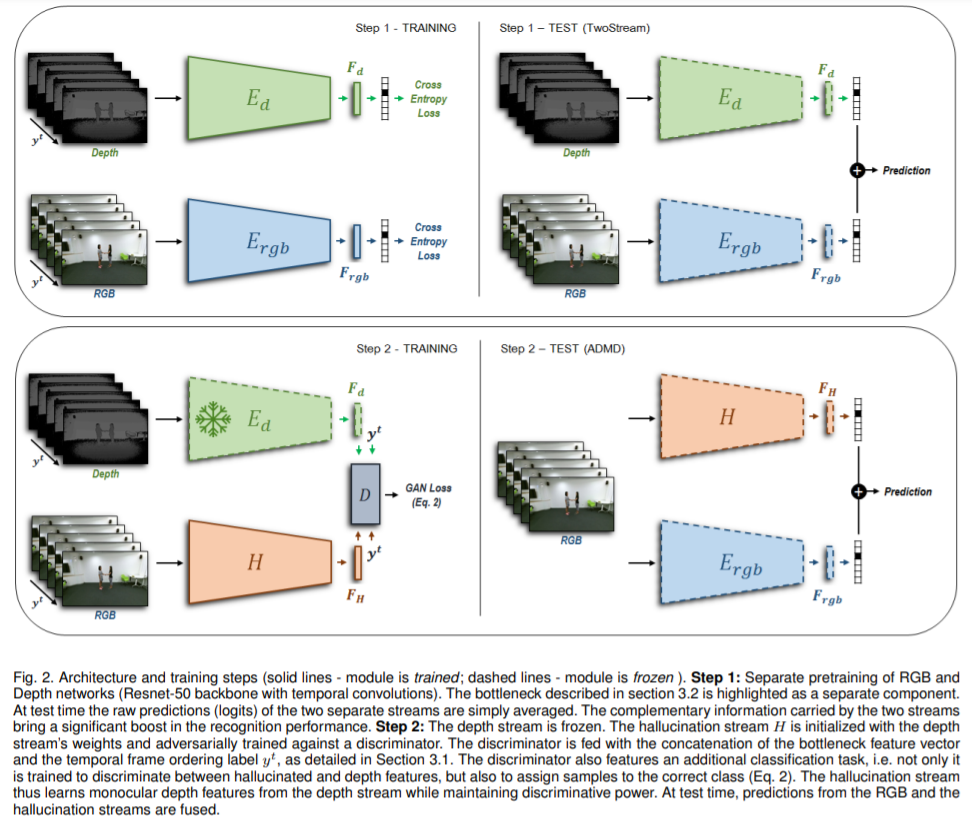
\includegraphics[width=0.80\textwidth]{img/c1m2.png} 
\caption{论文图 2}
\label{Test}
\end{figure}

图 2. 架构和训练步骤 (实线 - 模块被训练;虚线 - 模块被冻结),第 1 步:单独预训练 RGB 和深度网络(具有时间卷积的 Resnet-50 主干),第 3.2 节中描述的瓶颈突出显示为一个单独的组件,在测试时的两个独立流的原始预测(logits)被简单地平均,两个流携带的互补资讯带来了识别性能的显著提升。

步骤 2:深度流被冻结,幻觉流 H 用深度流的权重初始化,并针对鉴别器进行对抗训练。其鉴别器由瓶颈特征向量和时间帧排序标签 $y^{t}$ 的串联提供,如第 3.1 节所述。

鉴别器还具有额外的分类任务,即不仅训练它区分幻觉特征和深度特征,而且还将样本分配给正确的类 (等式 2),因此幻觉流从深度流中学习单眼深度特征,同时保持判别能力,在测试时,融合了来自 RGB 和幻觉流的预测,在标准对抗训练中,鉴别器 D 会尝试将二进制标签真/假分配给来自两个不同流的特征向量。然而我们发现用这种机制生成的特征 $F_{H}$ 尽管混合得很好并且与 $F_{d}$ 无法区分,但在分类任务中很难达到良好的准确性,即缺乏辨别力。

出于这个原因,我们为鉴别器分配了辅助任务,即用正确的类别对特征向量进行分类。

对抗性学习问题形式化如下。

考虑 RGB-D 数据集 $(X_{rgb}, X_{d}, Y )$,其中 $x^{t}_{rgb}, x^{t}_{d} (X_{rgb}, X_{d}, Y)$ 是时间对齐的 RGB 和深度帧,y ~ Y 是类标签的 C 维单热编码, C 是手头问题的类数。现在让扩展标签向量具有 C+1 个组件(类):

$$
\hat{y}= \begin{cases}{[z \operatorname{eros}(C) \| 1],} & \text { for } x_{r g b} \\ {\left[y_{i} \| 0\right]} & \text { for } x_{d}\end{cases}
$$

其中 zeros(C) 表示维度为 C 的零向量,并且 || 是连接运算符,在鉴别器中使用这个标签向量而不是经典的 0/1 (真实/生成)二元标签鼓励 H 学习的特征表示 FH 不仅编码深度 (单目)特征,而且具有判别性,这可能就是为什么幻觉网络经常能恢复老师的准确率,有时甚至表现得更好的原因,如实验部分进一步讨论的那样。

总之,我们希望 $F_{H}$ 特征与真实特征一样具有判别力:对抗性过程产生的假特征不仅被判别器归类为真实特征,而且还被分配到正确的类别,基于以上定义,我们定义了以下极大极小博弈:

$$
\begin{aligned}
\min _{\theta_{D}} \max _{\theta_{H}} \ell &=\mathbb{E}_{\left(x_{i}, y_{i}\right) \sim\left(X_{r g b}, Y\right)} \mathcal{L}\left(D\left(H\left(x_{i}\right) \| y^{t}\right), \hat{y}_{i}\right) \\
&+\mathbb{E}_{\left(x_{i}, y_{i}\right) \sim\left(X_{d}, Y\right)} \mathcal{L}\left(\mid D\left(E_{d}\left(x_{i}\right) \| y^{t}\right), \hat{y}_{i}\right)
\end{aligned}
$$

其中 $\theta_{H}$ 和 $\theta_{D}$ 表示幻觉流 H 和鉴别器 D 的参数,|| 表示连接操作,L 是 softmax 交叉熵函数。等式 2 通过众所周知的 ”label flipping hack”进行优化,这使得损失函数在实践中更容易最小化。

2. 建筑细节 (Architectural details) 

所有三个网络 (深度流 - $E_{d}$、RGB 流 - $E_{rgb}$ 和幻觉流 H) 都经过修改后的 Resnet-50 ,该方法增加了时间卷积并赋予了最终的瓶颈层。幻觉网络 H 使用各自的深度流权重 $E_{d}$ 进行初始化,遵循 J. Hoffman et al. 用于对象检测和 N. Garcia et al. 用于动作识别的发现。

(1) 时间卷积 (Temporal convolutions)

在 C. Feichtenhofer et al. 最近的工作之后,一维时间卷积被插入到每个 ResNet 层的第二个残差单元中,如图 3 所示,对于第 l 层,权重 $W_{l} \in \mathbb{R}^{1 \times 1 \times 3 \times C_{l} \times C_{l}}$ 是卷积滤波器,在特征级别初始化为身份映射,并以时间为中心,其中 $C_{l}$ 是第 $l$ 层中的通道数。更详细地说,$W_{l}$ 中包含的所有 [1 X 1 X 3] 时间内核都被初始化为 [0, 1, 0],即在开始时仅使用中心帧的资讯。随着训练的进行,这种情况会逐渐改变。最近在 D. Tran et al. 中,作者使用时间卷积探索了各种网络配置,比较了影像分类任务的不同组合。这项工作表明,将 3D 卷积解耦为 2D (空间) 和 1D (时间)滤波器是动作识别任务中的最佳设置,可产生最佳精度,而后一种设置的直觉是在两个连续的卷积层中分解空间和时间卷积可以简化空间和时间任务的训练 (也符合 L. Sun et al.)。

(2) 瓶颈 (Bottleneck) 

由于 GAN 极小极大游戏定义的鞍点固有的不稳定性,通过对抗训练生成、编码或对齐高维特征向量通常是一项艰巨的任务,出于这个原因 R. Volpi et al. 建议对齐一个较低维的向量,这是通过向标准架构添加瓶颈层而获得的。这通常不会影响基线模型的性能。实际上,最后一个 ResNet-50 层 (在 logits 之前)的大小是 [7, 7, 2048],或者在池化之后只是[2048]。

出于这个原因,我们通过添加任何一个方式来进一步修改 ResNet-50 ,i) 一个额外的卷积层,其权重 $W_{b} \in \mathbb{R}^{7 \times 7 \times 2048 \times 128}$,应用无填充,将维度降低到 128; 或者在 ii) 池化后的一个简单的 128 维全连接层。在原论文的第 4.2.1 节中,我们进一步探讨了瓶颈的选择。

(3) 输入 (Input) 

对于动作识别任务,编码器网络 E 和 H 的输入是五个 3 通道帧,从每个影像序列中均匀采样,这会激发时间卷积。相反来说,对于来自单个图像的对象分类任务,其架构中没有添加时间内核。我们为深度通道尝试了不同的编码:对于动作识别任务,它们使用喷射颜色图编码成彩色图像,如 A. Eitel et al. 对于物体识别任务,所考虑的资料集中已经提供了 HHA 编码 S. Gupta et al.。

(4) 鉴别器 (Discriminator) 

用于玩对抗游戏的鉴别器根据任务具有不同的架构,而这些架构遵循对抗性学习文献中经过经验验证的常见实践,更具体地说是 R. Volpi et al. 中描述的内容。它的基本结构是多层感知器,仅堆叠全连接 (fc) 层,因为它以向量作为输入 (瓶颈特征,可能与涉及时间的任务的时间顺序连接)。对于动作识别任务,结构相当浅,包括 D1=[fc(2048), fc(1024), fc(C+1)]。对于对象分类的任务,结构反而更复杂 D2=[fc(1024), fc(1024), fc(1024), fc(2048), fc(3072), fc(C+1)], with skip 低层的连接。作为非常深的前鉴别器,插入了残差连接以允许梯度流过底层的幻觉流,而架构的细节如图 4 所示。

\begin{figure}[htb]
\centering 
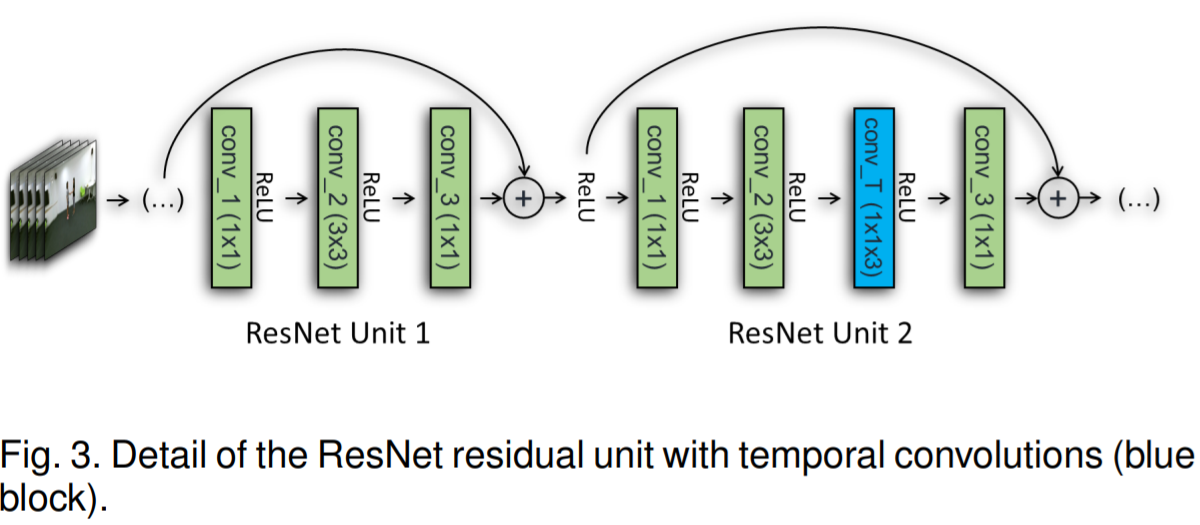
\includegraphics[width=0.80\textwidth]{img/c1m3.png} 
\caption{论文图 3}
\label{Test}
\end{figure}

图 3. 带有时间卷积的 ResNet 残差单元的细节 (蓝色块)。

\subsection{实验}
% 4 EXPERIMENTS 实验

1. 资料集 (Datasets) 

我们评估了我们的方法在一个对象分类和两个影像动作分类资料集上的性能,而对于这两个任务,模型都使用 ImageNet 预训练权重进行初始化。对于在较小的动作识别资料集 NW-UCLA 上的实验,我们从在较大的 NTU RGB+D 资料集上训练的 RGB 和深度流开始对模型进行微调。

(1) NTU RGB+D

我们评估了我们的方法在一个对象分类和两个影像动作分类资料集上的性能,而对于这两个任务,模型都使用 ImageNet 预训练权重进行初始化。对于在较小的动作识别资料集 NW-UCLA 上的实验,我们从在较大的 NTU RGB+D 资料集上训练的 RGB 和深度流开始对模型进行微调。

\begin{figure}[htb]
\centering 
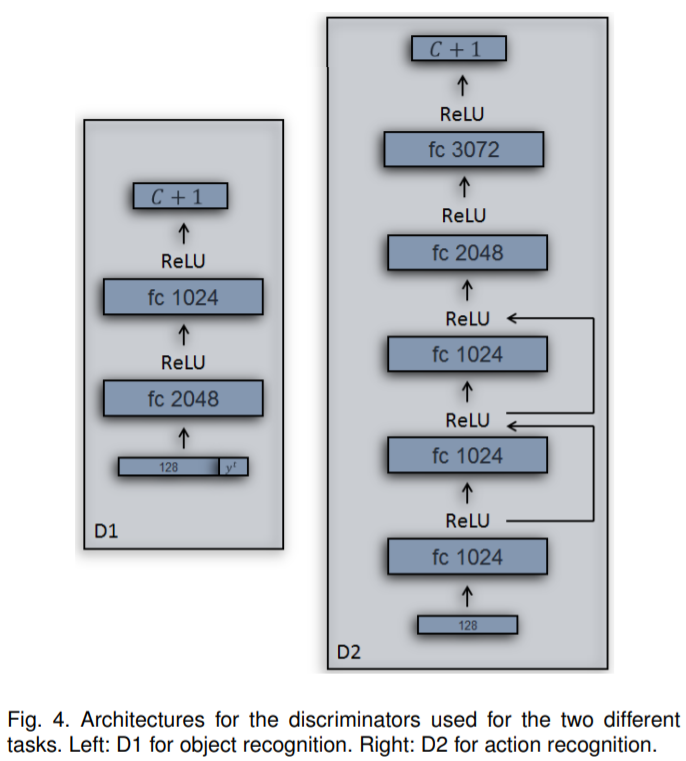
\includegraphics[width=0.80\textwidth]{img/c1m4.png} 
\caption{论文图 4}
\label{Test}
\end{figure}

图 4. 用于两个不同任务的鉴别器的架构。左:用于物体识别的 D1。右:用于动作识别的 D2。

\begin{figure}[htb]
\centering 
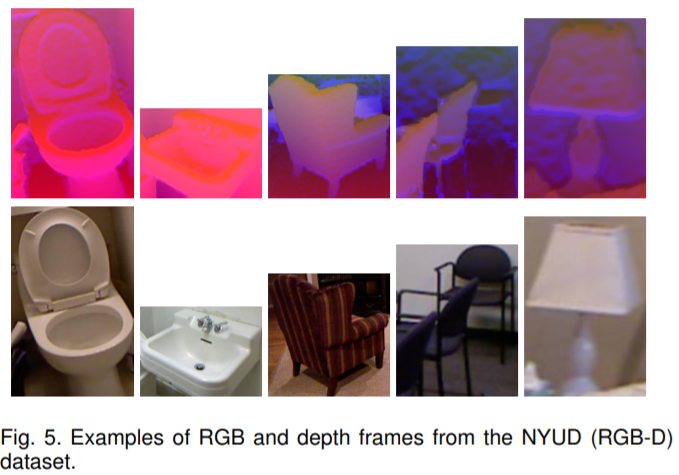
\includegraphics[width=0.80\textwidth]{img/c1m5.png} 
\caption{论文图 5}
\label{Test}
\end{figure}

图 5. 来自 NYUD (RGB-D) 资料集的 RGB 和深度帧示例。

\begin{figure}[htb]
\centering 
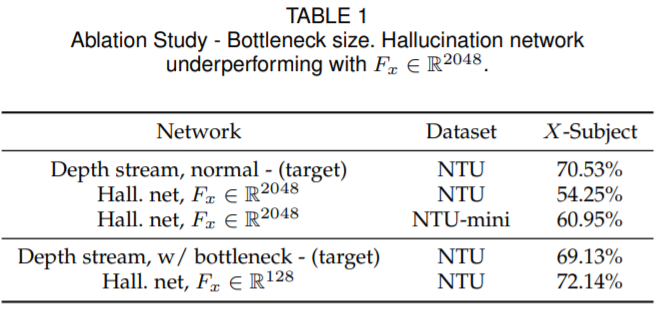
\includegraphics[width=0.80\textwidth]{img/c1m6.png} 
\caption{论文表 1}
\label{Test}
\end{figure}

TABLE 1-表格 1 消融研究 - 瓶颈尺寸。幻觉网络在 $F_{x} \in \mathbb{R}^{2048}$ 上表现不佳。

(2) Northwestern-UCLA

这个动作识别资料集提供了 1475 个样本的 RGB、深度和骨架序列,它有 10 个主体执行 10 个动作,在 3 个不同的视图中捕获。

(3) NYUD (RGB-D)

该对像资料集 (参见图 5 中的示例) 是通过在 N. Silberman et al. 的 NYUD 资料集中存在的 19 个对像类的实例周围裁剪出紧密边界框来收集的,它包括 2,186 张成对的标记训练图像和 2,401 张测试图像 (RGB-D)。深度图像是 HHA 编码的 S. Gupta et al.,而此版本的资料集是在 J. Hoffman et al. 中提出的,但也在 R. Volpi et al.、 E. Tzeng et al.、P. Morerio et al. 中用于模态适应的任务,在域适应的框架内,也就是在一种模态上训练,适应和测试模型 在另一种方式上。这里的任务是对象分类、两种模式的训练和仅在 RGB 上的测试。

2. 消融研究 (Ablation Study) 

消融研究是在 NTU RGB+D 资料集的一部分上进行的,指定为 mini-NTU,它由来自训练集的随机样本组成,考虑到原始资料集大小的大约三分之一,测试集仍然与其他实验中使用的相同,最初在 A. Shahroudy et al. 中定义。我们研究了幻觉网络性能如何受到以下因素的影响:(1)向鉴别器提供不同类型的输入,以及(2)让鉴别器执行不同的任务。

(1) 瓶颈大小 (Bottleneck size) 

鉴别器分别接收来自幻觉或深度流的特征向量 $F_{H}$ 或 $F_{d}$ 作为输入,以及帧索引标签 $y^{t}$,众所周知,太大的特征向量可能会导致 GAN 训练表现不佳  R. Volpi et al. ,我们在实验中也观察到了这一点,如表 1 所示。我们首先在完整的 NTU 资料集上无瓶颈地训练了我们的深度网络,达到了 70.53\% 的准确率,然后将该网络用作学习幻觉模型的目标。我们观察到没有瓶颈训练的幻觉模型,即判别器的输入是 2048 维特征向量,远没有恢复目标的性能(仅达到 54.25\%),即使训练空间减少到 NTU-mini 资料集 (60.95\%),然后我们训练一个具有 128 维瓶颈 (69.13\%) 的网络,使用之前的深度流初始化,除了使用 MSRA 初始化随机初始化的瓶颈 K. He et al.,使用瓶颈特征向量学习的幻觉模型不仅能够恢复,而且能够超越深度流的性能,达到 72.14\% 的准确率。我们在论文中的其他实验中观察到了这种行为,我们在后面的 4.4 节中对此进行了评论。

(2) 瓶颈实施 (Bottleneck implementation) 

在表 2 中,我们研究了将 $F_{x}$ 的大小从 $\mathbb{R}^{2048}$ 减小到 $\mathbb{R}^{128}$ 的不同方法,如  R. Volpi et al. 中所建议的,在最后一个维度为 7*7*2048 的特征图之后,我们测试了以下三种方式:

在表 2 中,我们研究了将 $F_{x}$ 的大小从 $\mathbb{R}^{2048}$ 减小到 $\mathbb{R}^{128}$ 的不同方法,如  R. Volpi et al. 中所建议的,在最后一个维度为 7*7*2048 的特征图之后,我们测试了以下三种方式:

\begin{itemize}

\item [-][128,7,7] 卷积到 1*1*128

\item [-][7,7] 空间卷积到 1*1*2048 然后一维卷积到 1*1*128

\item [-]池化层到 1*1*2048 然后一维卷积到 1*1*128

\end{itemize}

\begin{figure}[htb]
\centering 
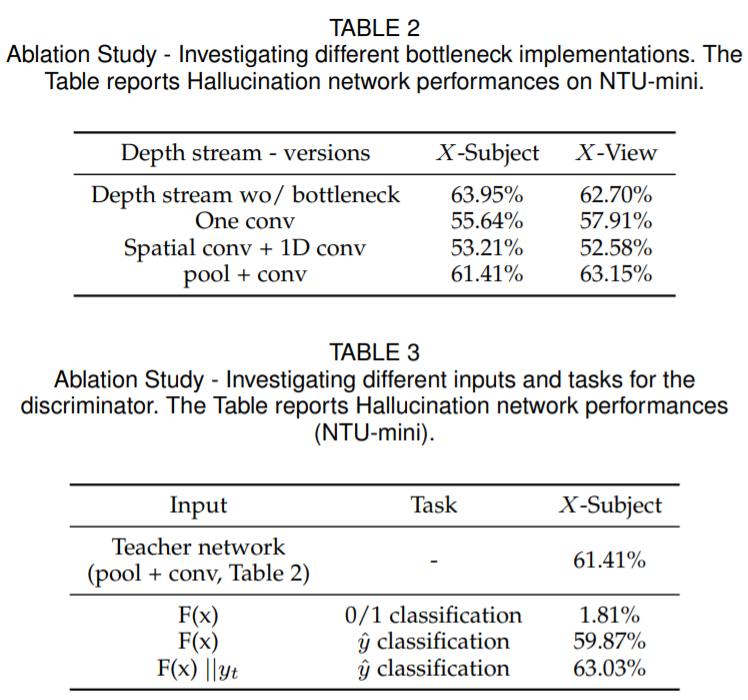
\includegraphics[width=0.80\textwidth]{img/c1m7.png} 
\caption{论文表 2 和 3}
\label{Test}
\end{figure}

TABLE 2 表 2
消融研究 - 调查不同的瓶颈实施,该表报告了 NTU-mini 上的幻觉网络性能。

TABLE 3 表 3
消融研究 - 调查鉴别器的不同输入和任务,该表报告了幻觉网络性能 (NTU-mini)。即使深度流只是在 NTU-mini 上训练(跨学科 63.95\%,交叉视角 62.70\%),实现 pool+conv 瓶颈的幻觉流几乎可以完全恢复(跨学科 61.41\%),甚至超过(63.15\% for cross view),原始深度流性能。这是我们在其余实验中使用的架构选择。

%\begin{itemize}
%\item Calculus
%\item Linear Algebra
%\item Basic Computer Concepts
%\end{itemize}

%\begin{description}
% \item[First] \hfill \\
% The first item
% \item[Second] \hfill \\
% The second item
% \item[Third] \hfill \\
% The third etc \ldots
%\end{description}

(3) 鉴别器:输入和任务 (Discriminator: inputs and tasks)

在本节中,我们探讨分配给鉴别器的任务是否会影响幻觉表现。

如第 3 节所述,我们的假设是生成器的艰巨任务是生成不仅与深度特征相对应的特征,而且还需要在时间上与这些特征配对。

我们通过引入帧索引 $y^{t}$ 的附加资讯来解决这个问题,它指定了所需的对齐方式。

表 3 显示了关于

(1) 以特征瓶颈作为输入的 GAN 生成器的传统二元任务,

(2) $\hat{y}$ 分类任务具有与之前相同的输入,以及

(3)建议的方法。

传统的二元任务 (1) 收敛到一个完美的平衡点,但幻觉流的准确性接近随机概率,这意味着学习到的特征根本没有判别力。

第二种方法 (2) 能够学习判别特征,但添加帧顺序监督 $y_{t}$ (3) 显示了性能的提高。

由于对时间卷积的更高依赖性,这种机制在更具挑战性和多样性的资料集上产生最大化收益是合理的,如完整的 NTU 资料集,或在全 3d 卷积架构 (如 I3D  J. Carreira et al.)中。

3. 动作识别性能及比较 (Action recognition performance and comparisons) 
表 4 比较了文献中不同方法在动作识别的两个数据集上的性能—NTU RGB+D 和 NW-UCLA 的两个协议。用于此任务和资料集的标准性能度量是分类准确度,根据各自作品中定义的协议、训练和测试拆分进行估计。表格的第一部分(用符号表示)指的是无监督方法,即使在学习表示中不依赖标签,也能取得惊人的高结果。第二部分是监督方法(用 4 表示),根据用于训练和测试的方式进行划分。在这里,我们报告了在步骤 1(第 7 行和第 8 行)中训练的单独 RGB 和深度(有和没有瓶颈)流的性能,性能的小幅提升可能是由于在 mini-NTU(用于消融研究)上训练的瓶颈版本初始化后,额外的训练步骤和小学习率。而重要的是,具有瓶颈的深度流代表用于幻觉学习的教师网络。我们希望我们的最终模型比仅在 RGB 上训练的模型表现更好,其准确性构成了我们的幻觉模型有用性的下限,为 NW-UCLA 资料集的第 1 步模型报告的值,即 RGB 和深度流,指的是我们 NTU 模型的微调。

而 N. Garcia et al. 相比,为了更清晰的分析,双流设置始终没有进行微调,它的准确度代表了最终模型的上限,它不会依赖于测试时的深度资料,我们已经尝试使用预训练的 ImageNet 权重代替 NTU 进行训练,但它导致了较低的准确率。表格的最后一部分 (用□表示)报告了特权资讯框架中方法的性能,因此可以直接与我们的进行比较,参考 Hoffman 等人的性能值。方法 J. Hoffman et al. (表 4 的第 20 行)取自  N. Garcia et al. 中的实施和实验。第 21 行引用了 Luo 及其同事 Z. Luo et al. 的方法,该方法在训练时使用 6 种模态 (RGB、深度、光流和骨架资料的三种不同编码方法),而在测试时仅使用 RGB。而 N. Garcia et al. 的第 3 步和第 4 步 (第 22 行和第 23 行)分别参考了幻觉学习及其微调后的双流模型。我们注意到,为了简单起见,ADMD Two-Stream 模型的结果仅仅是两个流的 logits 的平均值的结果,并且没有经过任何微调,这意味着它们可以直接与第 22 行进行比较。

此外,第 24 行的结果仅对应于幻觉流,我们注意到幻觉流(第 24 行)设法恢复并超过了 NW-UCLA 资料集的深度教师流(第 8 行)(83.94\% 与 71.09\% 相比),而对于 NTU p1(67.57\%) 和 p2 (71.80\%) 协议比各自的教师 (71.87\% 和 75.32\%)低约 4\%。然而,当与 RGB 流结合时,它的性能更好 (NTU p2 - 81.50\%) 或与 N. Garcia et al. 中提出的微调模型相当 (NTU p1 - 73.11\%)。由于 RGB 流在这项工作和 N. Garcia et al. 中的表现同样出色,我们可以得出结论,性能的提高是由于更好的幻觉特征。

4. 物体识别性能和比较 (Object recognition performance and comparisons) 

表 5 说明了 NYUD 资料集在对象识别任务中获得的主要结果与动作识别相反,这里的深度资讯通常是嘈杂的 (参见图 5 - 椅子和灯),可能是由于边界框裁剪的分辨率小。事实上,单独的深度比单独的 RGB 表现更差 (超过 10\% 的差距)。尽管如此,尽管深度性能很差,但当在双流模型中融合时,两种模态携带的互补资讯量能够将识别准确度提高 5 个百分点以上 $($ RGB $\rightarrow 52.90 \%$, Depth $\rightarrow 40.19 \% \Rightarrow$ two-stream $\rightarrow 57.39 \%)$。

\begin{figure}[htb]
\centering 
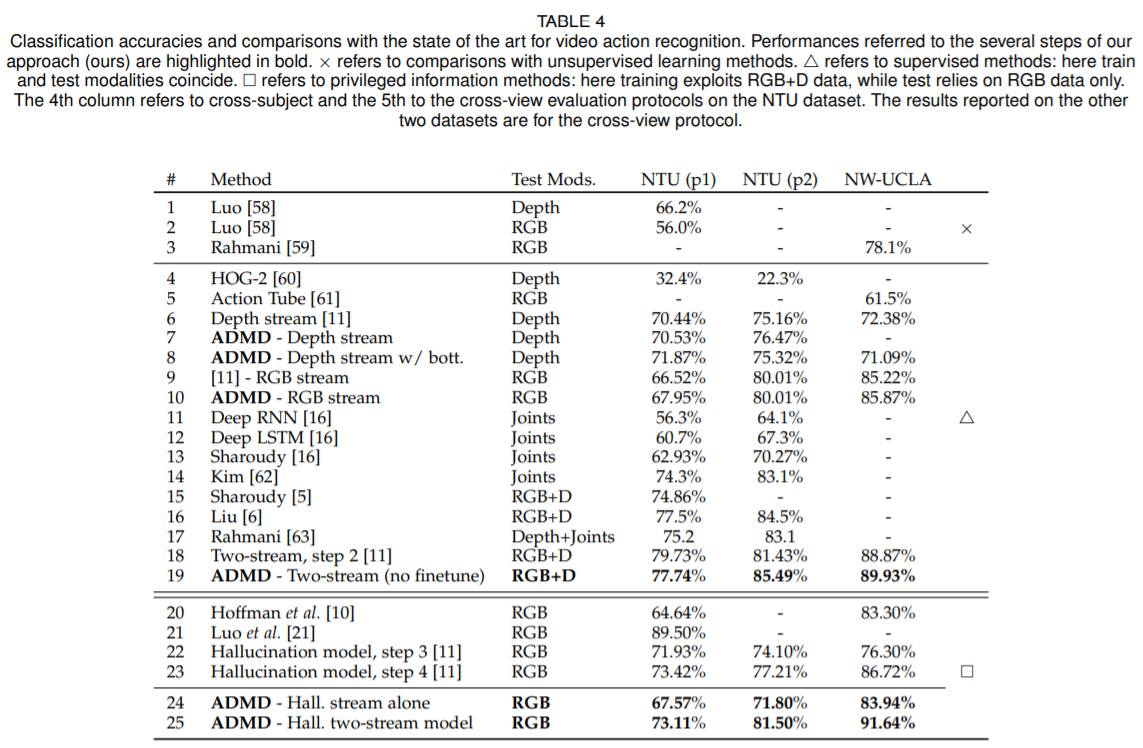
\includegraphics[width=0.80\textwidth]{img/c1m8.png} 
\caption{论文表 4}
\label{Test}
\end{figure}

TABLE 4 表 4
影像动作识别的分类精度和与现有技术的比较,涉及我们方法(我们的)的几个步骤的性能以粗体突出显示。指与无监督学习方法的比较,4 指的是监督方法:这里训练和测试模式一致。指特权资讯方法:这里的训练利用 RGB+D 资料,而测试仅依赖于 RGB 资料,第 4 列涉及跨学科,第 5 列涉及 NTU 资料集上的跨视图评估协议。在其他两个资料集上报告的结果是针对跨视图协议的。

\begin{figure}[htb]
\centering 
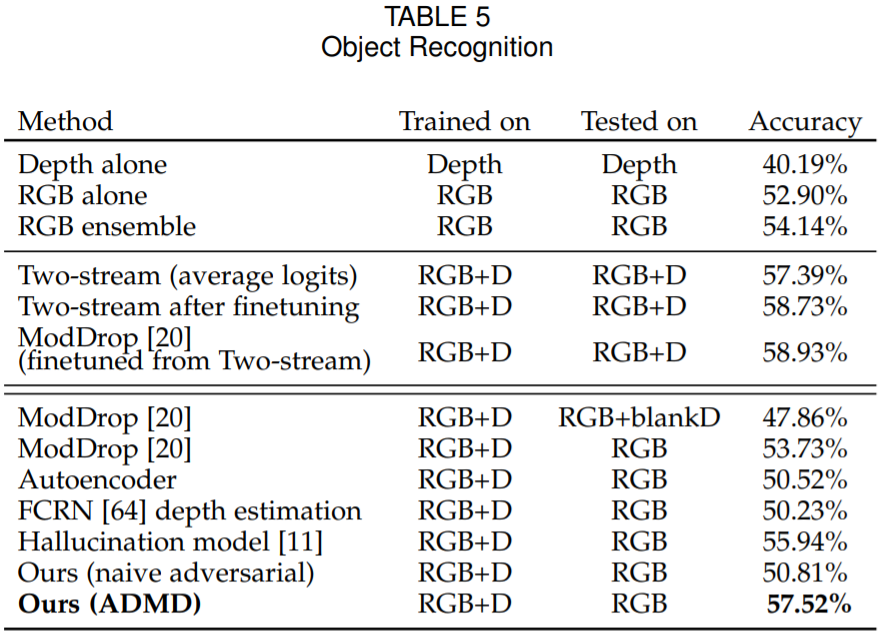
\includegraphics[width=0.80\textwidth]{img/c1m9.png} 
\caption{论文表 5}
\label{Test}
\end{figure}

TABLE 5
物体识别 (Object Recognition )


众所周知,集成方法往往优于其单一模型对应物:两个 CNN 的集成,每个 CNN 从不同的初始化开始训练,优于任一独立模型 J. Guo et al.,由于原则上提出的 ADMD 策略是使用标准监督方法训练的 RGB 模型和另一个对抗训练的 RGB 模型的组合,因此我们另外将我们的方法与 RGB 分类器的集合进行比较 (表 5 的第三行)。有趣的是,尽管从两个相对较高的单流性能开始,两个 RGB 网络的融合过程只是略微提高了最终的准确率 (RGB1 $\rightarrow 53.19 \%$, RGB2 $\rightarrow 52.60 \%$ $\Rightarrow$ Ensemble $\rightarrow 54.14 \%$ ).。

正如在动作识别任务中注意到的那样,我们发现微调融合流并不总是带来显著的改进,与 N. Garcia et al. 相反,架构具有跨流乘法器连接,需要进一步训练。使用 Neverova et al. 提出的策略进行微调看起来稍微更有效,因为 ModDrop 在输入层引入了光衰减,包括图像和整个模态。结果模型在  N. Neverova et al. 中提出的原始设置中进行了测试,即通过消隐深度流和简单地使用 RGB 预测。而后一种方案略微提高了 RGB 流的性能,这可能要归功于 dropout。然而,尽管该模型在测试时对缺失的深度表现出更强的鲁棒性(robustness),但它显然无法提取任何单眼深度线索。我们执行的另一个有趣的比较如下:我们训练一个具有 L2 损失的跨模态自动编码器,以便从 RGB 重建深度图,编码器解码器架构包括用于编码器的相同 RGB ResNet-50,以及用于解码器的与批规范层交织在一起的 5 个堆叠解卷积块。在测试时,当深度不可用时,我们向自动编码器提供 RGB 帧,自动编码器重建缺失的模态以馈送双流架构的相应分支,而这种设置的性能很差。


我们观察到自动编码器很容易过拟合训练集,为训练集生成高质量的深度图,而它在测试集上的表现却很差。同样,我们通过 FCRN I. Laina et al. 重建深度,这是一种在整个 NYUD 资料集上训练的最先进的深度估计器。性能很差,因为 FCRN 估计的深度错过了对象分类所需的许多精细细节。这表明对于识别任务来说,幻觉任务特定特征比估计深度更有效。 I. Laina et al. 中提出的幻觉模型的结果再次证实了这一说法,在这种情况下适用于对象识别 (表 5,第 3 行到最后一行),这种方法优于 RGB 流和 RGB 集成,证实了幻觉深度的价值。它还优于仅在测试时使用 RGB 的其他基线 (表 5 的第 3 部分)。特别是它的性能比 FCRN 深度估计要好得多,这再次表明深度特征幻觉比在像素级别预测深度图更有效。

更重要的是,我们可以直接将其与本文提出的 ADMD 进行比较 (55.94\% vs 57.52\%),得出的结论是与动作识别实验类似,对抗性方法表现更好。最终我们在两种不同的设置中测试了我们的对抗方案:i) 天真设置,其中鉴别器 D 仅被分配了二元任务,以及 ii) ADMD 设置,其中鉴别器也被分配了分类任务,前者作为自动编码器,后者能够完全恢复双流模型的精度,仅略低于微调模型的精度。


5. 带有噪声深度的推理 (Inference with noisy depth)

\begin{figure}[htb]
\centering 
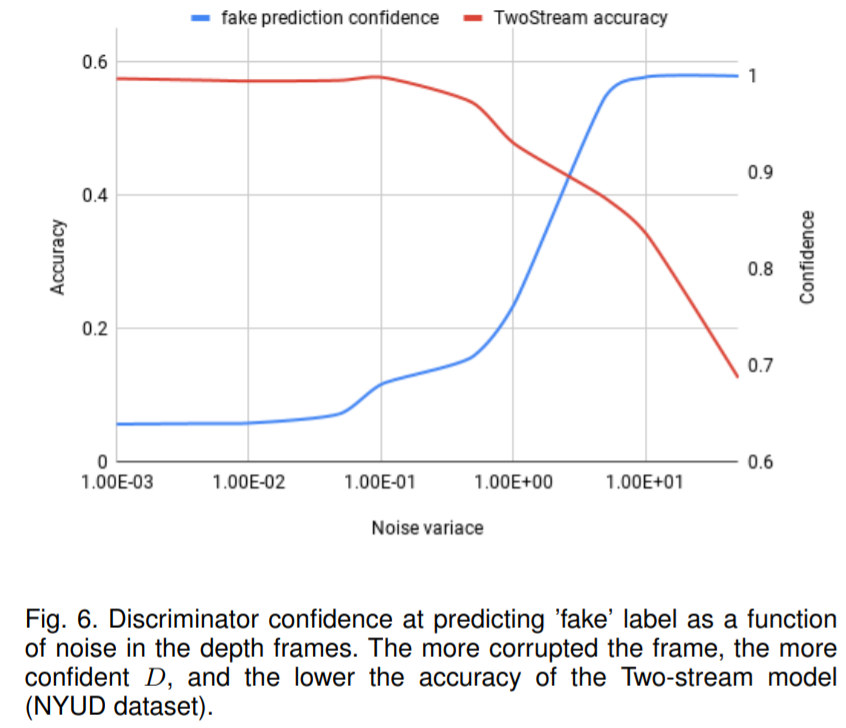
\includegraphics[width=0.80\textwidth]{img/c1m10.png} 
\caption{论文图 6}
\label{Test}
\end{figure}

图 6. 预测“假”标签作为深度帧中噪声函数的鉴别器置信度,而帧损坏越多,D 越有信心,双流模型(NYUD 资料集)的准确度就越低,而在真实的测试场景中,我们常常只能访问嘈杂的深度资料。

在本节中,我们将解决两个问题:i) 这种嘈杂的资料会在多大程度上降低多模式设置的性能? ii) 相对于使用带有噪声深度资料的教师模型 (Twostream) 而言,在哪个噪声水平上对深度模态产生幻觉更有利?
NTU 资料集 (Kinect) 中使用的深度传感器是一个 IR 发射器,与一个 IR 摄像头耦合,并且具有非常复杂的噪声表征,包括至少 6 个不同的源 T. Mallick et al.。研究影响深度通道的噪声模型超出了这项工作的范围,因此,对于我们的分析,我们选择影响最大的模型,即乘法散斑噪声。因此,我们在深度图像 I 中注入高斯噪声以模拟散斑噪声: $I=I * n, n \sim \mathcal{N}(1, \sigma)$

表 6 显示了当深度被这种随着方差增加的高斯噪声破坏时,我们的双流网络的性能如何下降 (NTU 交叉视图协议和 NYUD),结果表明,相对于表 4 中我们的幻觉模型 (81.50\% - 第 25 行) 保证的精度,即使 $\sigma^{2}=10^{-1}$ 的低噪声方差,精度也显著降低。对于对象识别的任务,我们可以看到 N. Neverova et al. 的 ModDrop 比简单的 Two-stream 更能适应深度损坏,因为在输入层中用噪声 (dropout) 进行了微调。总之该实验表明 ADMD 不仅能够处理缺失的模态,还能够处理嘈杂的模态。在在线场景中,在步骤 2 中训练的鉴别器 D 可以指示何时可操作地从双流切换到 ADMD,即何时用幻觉代替深度分支。当训练达到平衡时,D 被 H 生成的特征最大限度地愚弄,无法将它们与 $E_{d}$ 编码的特征区分开来。

在实践中,这意味着假类 ($\hat{y}$ 中的最后一个类,方程 1)的预测概率平均为 $p(\hat{y}=C+1) \approx .5$。然而,当从损坏的深度计算的特征开始流入 D 内部时,它对假类的预测开始越来越有信心。图 6 绘制了 D 随着噪声增加的行为以及双流模型的准确性。准确度和置信度都有一个明显的转折点,可以在实践中决定何时从 $E_{d}$ 切换到 H,即何时将深度作为一种模式并开始使用从 RGB 中提取的单眼深度特征。

6. 讨论 (Discussion) 

一些有趣的观点来自对我们发现的分析,我们在下面总结。

(1) RGB 和深度实际上携带补充资讯。

事实上,双流设置总是比单独使用两个流提供令人惊讶的更好的准确性。作为额外的证据,尽管其单流组件之一 (深度或 RGB,取决于任务和资料集) 的准确性较低,但多模态集合 (即双流) 的性能优于单模态集合 (表 5)。

(2) RGB 图像中有(单目)深度资讯。

从幻觉流经常恢复并且有时超过其基于深度的教师网络的准确性这一事实中可以明显看出这一点,此外融合幻觉和 RGB 流总是带来好处,如融合 RGB 和深度。


TABLE 6

在 RGB 和深度上训练的双流模型的准确度值,并使用 RGB 和噪声深度资料进行测试。

\begin{figure}[htb]
\centering 
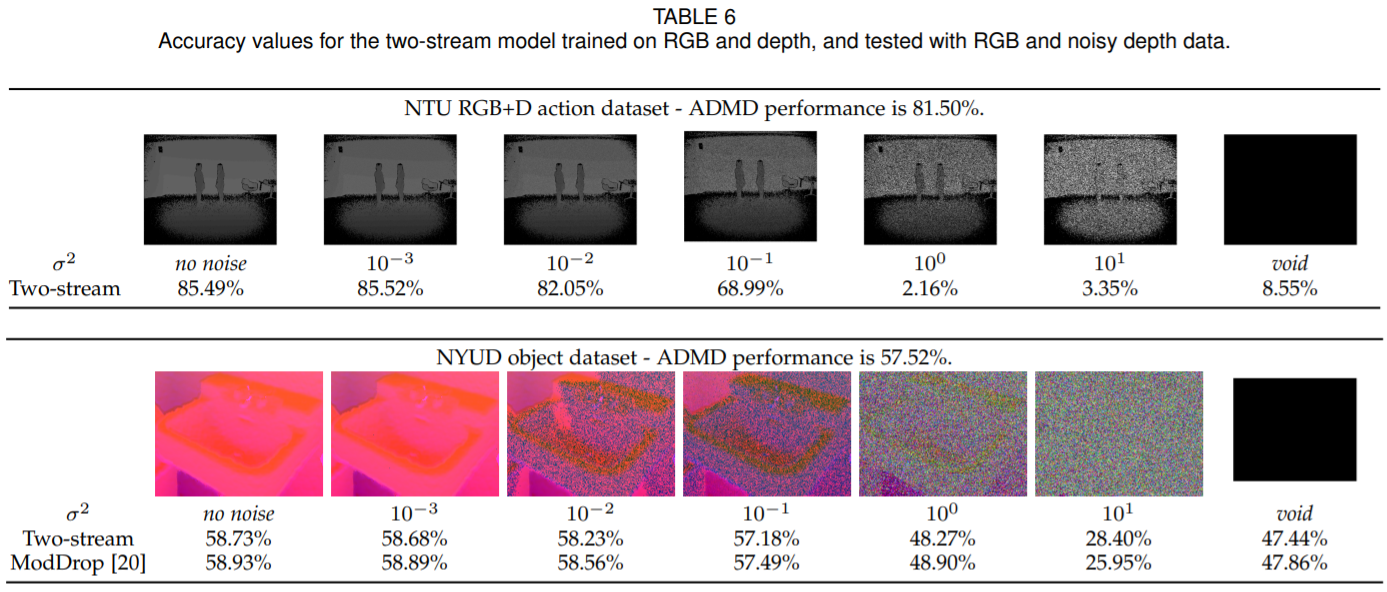
\includegraphics[width=0.80\textwidth]{img/c1m11.png} 
\caption{论文表 6}
\label{Test}
\end{figure}

(3) 标准监督学习在提取资讯方面存在局限性。

事实上,鉴于有证据表明 RGB 图像中存在可利用的深度资讯,最小化交叉熵损失并不足以完全提取它。为此,我们需要一个学生-教师对抗框架。这在对抗性网络压缩 V. Belagiannis et al. 中有一个有趣的相似之处,其中完全监督的小型网络的性能可以通过对抗高容量 (和更好性能) 教师网络的对抗性训练来提高。在 V. Belagiannis et al. 中,还观察到学生在某些情况下可以超越老师。

(4) 仅靠对抗训练是不够的。

为二元任务 (真实/生成) 训练的朴素判别器不足以迫使幻觉网络产生判别特征。辅助判别任务对于提取对给定任务也具有判别力的单眼深度线索是必要的 (另一方面,仅辅助任务是不够的,正如 RGB 集成的性能所暗示的那样)。

(5) 幻觉特定于任务的深度特征比估计全深度图像更有效。

不仅估计的深度通常缺少分类所需的细节,而且其估计仅由重建目标驱动,相反的特征幻觉解决了特定的分类任务,需要估计低维向量而不是图像。

\subsection{结论}
% 5 CONCLUSIONS 结论

在这项工作中,我们引入了一种新技术来利用额外资讯,在训练时以深度图像的形式,在测试时改进仅 RGB 模型。这是通过对抗性训练幻觉网络来完成的,该网络从教师深度流中学习如何从 RGB 帧编码单眼深度特征。在三个不同资料集的对象分类和动作识别任务中,所提出的方法在特权资讯场景中优于以前的方法。此外,幻觉框架在深度嘈杂的情况下非常有效。

Code is available at (https://github.com/pmorerio/admd).
	\chapter{研究工具与手段的分类}
\label{chap:2}



\begin{itemize}
\item [-] XXX
\end{itemize}


\begin{figure}[htb]
\centering 
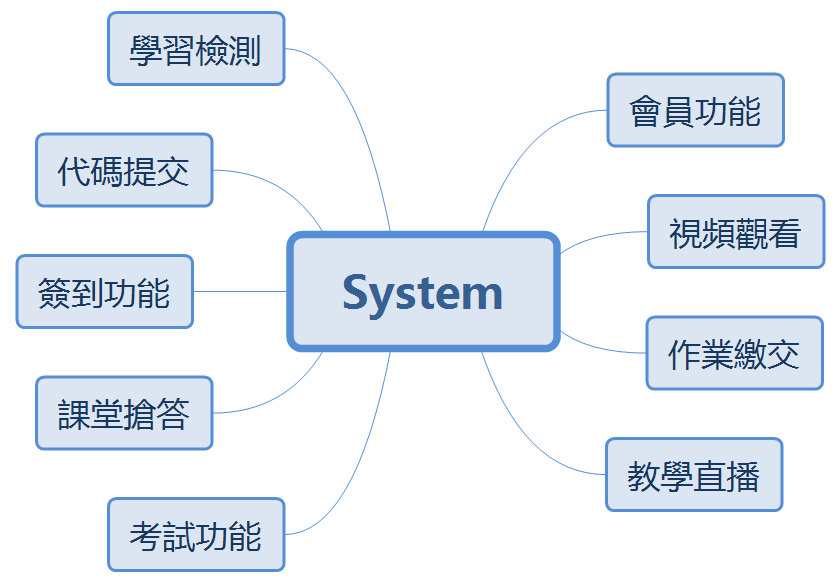
\includegraphics[width=0.90\textwidth]{img/ch1m1.png} 
\caption{官网}
\label{Test}
\end{figure}

    
    \appendix
    \printbibliography[heading = bibintoc]
    
    % 如有需要使用研究生成果页
    \def\cpublication{攻读硕士期间发表的论文及其他成果}

%\renewcommand{\bibname}{\cpublication}
%\begin{thebibliography}{9}{
%\zihao{5}
%\bibitem{publish} 
%\textbf{扎克·施耐德}, XXX XXX, et al. XXXX Title[C/OL]//III H D, SINGH A. Proceedings of Machine Learning Research: Proceedings of the 37th International Conference on Machine Learning: vol. 119. [S.l.]: PMLR, 2020: XXXX-XXXX. http://proceedings.ml r.press/XXXX.html.(一作,CCF-A)
%}\end{thebibliography}
%\addcontentsline{toc}{chapter}{\cpublication}


	\backmatter
	\chapter{致谢}

非常感谢 刘宏 教授,在  课让XXXXXX,该工作也帮助到学生目前的开发与研究工作进度,同时也对目前深度伪造的进展有所调研,同时也将此流程在其他课程的作业上进行测试获得良好的回馈。最后感谢在这一年来一起寒窗苦读得同学与所有老师,还有默默在开源社群与前沿研究奉献的技术人员跟研究者们。
	% 需替换门户原创页pdf/扫描pdf
	%% Copyright (c) 2008-2009 solvethis
% Copyright (c) 2010-2017,2021 Casper Ti. Vector
% Copyright (c) 2021 Kurapica
% Copyright (c) 2021 iofu728
% All rights reserved.
%
% Redistribution and use in source and binary forms, with or without
% modification, are permitted provided that the following conditions are
% met:
%
% * Redistributions of source code must retain the above copyright notice,
%   this list of conditions and the following disclaimer.
% * Redistributions in binary form must reproduce the above copyright
%   notice, this list of conditions and the following disclaimer in the
%   documentation and/or other materials provided with the distribution.
% * Neither the name of Peking University nor the names of its contributors
%   may be used to endorse or promote products derived from this software
%   without specific prior written permission.
%
% THIS SOFTWARE IS PROVIDED BY THE COPYRIGHT HOLDERS AND CONTRIBUTORS "AS
% IS" AND ANY EXPRESS OR IMPLIED WARRANTIES, INCLUDING, BUT NOT LIMITED TO,
% THE IMPLIED WARRANTIES OF MERCHANTABILITY AND FITNESS FOR A PARTICULAR
% PURPOSE ARE DISCLAIMED. IN NO EVENT SHALL THE COPYRIGHT HOLDER OR
% CONTRIBUTORS BE LIABLE FOR ANY DIRECT, INDIRECT, INCIDENTAL, SPECIAL,
% EXEMPLARY, OR CONSEQUENTIAL DAMAGES (INCLUDING, BUT NOT LIMITED TO,
% PROCUREMENT OF SUBSTITUTE GOODS OR SERVICES; LOSS OF USE, DATA, OR
% PROFITS; OR BUSINESS INTERRUPTION) HOWEVER CAUSED AND ON ANY THEORY OF
% LIABILITY, WHETHER IN CONTRACT, STRICT LIABILITY, OR TORT (INCLUDING
% NEGLIGENCE OR OTHERWISE) ARISING IN ANY WAY OUT OF THE USE OF THIS
% SOFTWARE, EVEN IF ADVISED OF THE POSSIBILITY OF SUCH DAMAGE.

{
	\ctexset{section = {
		format+ = {\centering}, beforeskip = {40bp}, afterskip = {15bp}
	}}
	\specialchap{北京大学学位论文原创性声明和使用授权说明}

	% 学校书面要求本页面不要页码,但在给出的 Word 模版中又有页码。
	% 此处以学校书面要求为准。
	\thispagestyle{empty}
	
	% 替换扫描pdf,去除includegraphics前注释
	\begin{textblock}{1}(-0.8,-0.08)
		\colorbox{white}{
			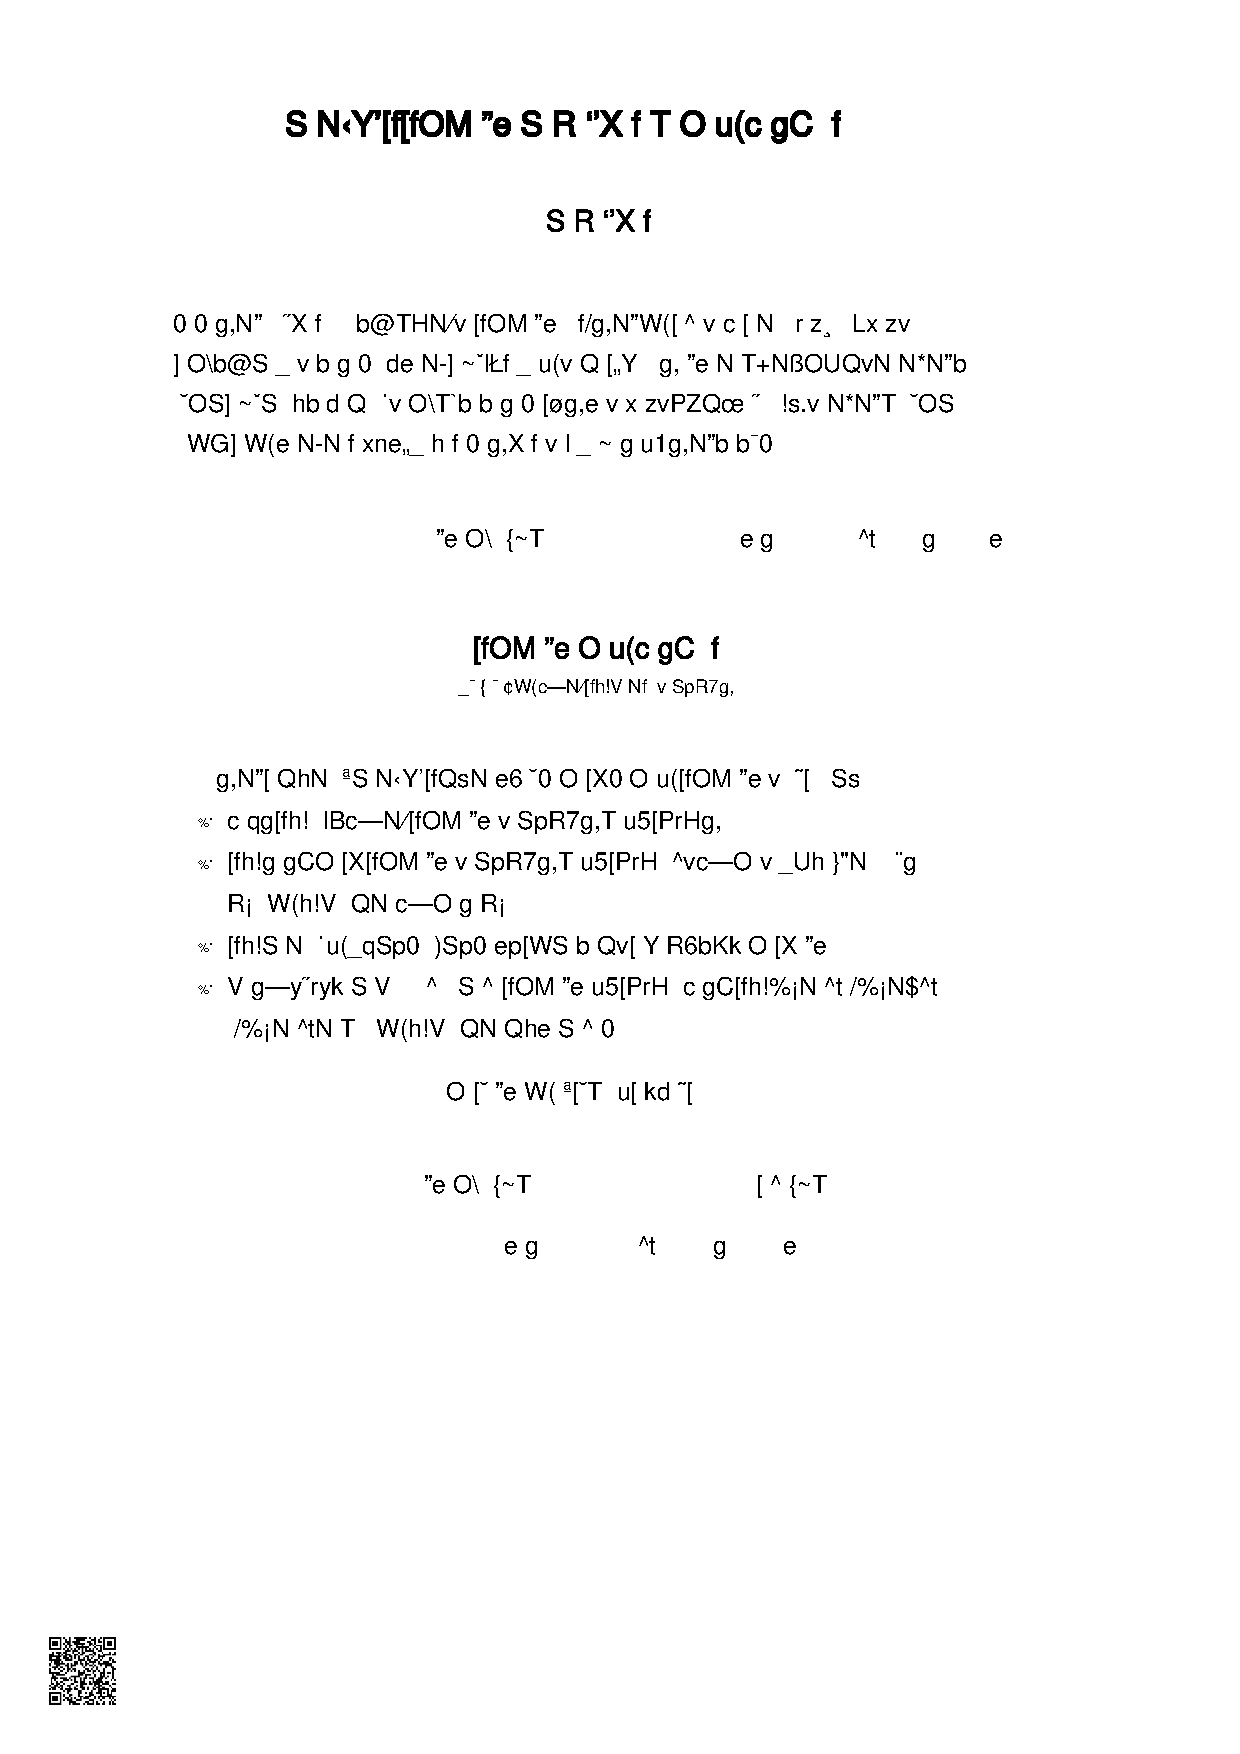
\includegraphics[height = 1.2448\textheight]{img/lwsm_180xxxxxxx.pdf}
		}
	\end{textblock}
}

% vim:ts=4:sw=4

\end{document}

% vim:ts=4:sw=4